\begin{frame}
   \frametitle{Talk Outline}
   \begin{tikzpicture}[font=\small]
      \tikzset{>=latex} % arrow heads
      \draw[step=1,black!15,very thin,opacity=\gridopacity] (0,0) grid (12,8);

      \node[fill=blue!15,minimum width=11cm] at (6,7.5) {\strut How to Optimize?};

      \node[fill=black!3,minimum width=5cm,minimum height=3cm] (lazysp) at (3.25,5.6) {};
      \node[anchor=north] at (lazysp.north) {\strut Lazy Pathfinding};
      \node[draw=black!30,fill=white,inner sep=5pt] at (3.25,5.4) {
         \includegraphics[width=3.8cm]{build/lazysp-icon}};

      \node[fill=black!3,minimum width=5cm,minimum height=3cm] (ibid) at (8.75,5.6) {};
      \node[anchor=north] at (ibid.north) {\strut Dynamic Pathfinding};
      \node[draw=black!30,inner sep=0pt] at (8.75,5.4) {
         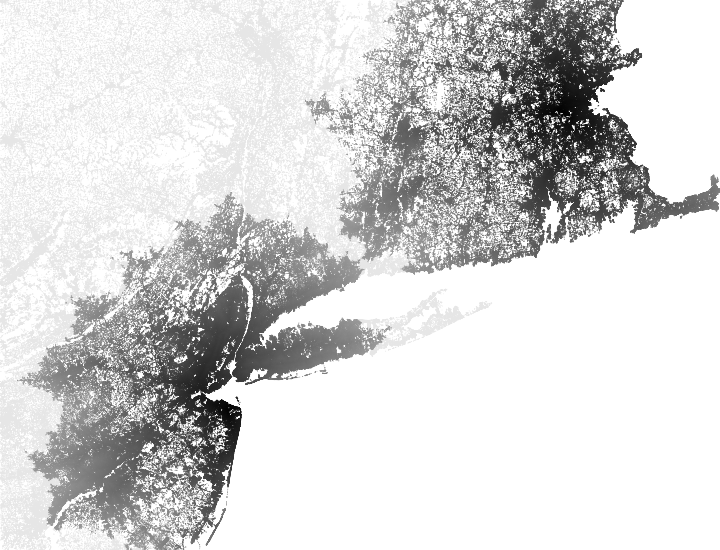
\includegraphics[width=2.9cm]{figs/incbi-road-ne/singleshot/example-bidijkstra.png}};

      \node[fill=blue!15,minimum width=11cm] at (6,3.5) {\strut What to Optimize?};

      \node[fill=black!3,minimum width=5cm,minimum height=3cm] (utility) at (3.25,1.6) {};
      \node[anchor=north] at (utility.north) {\strut Maximizing Utility};
      \node at (3.25,1.35) {\includegraphics[width=2.5cm]{build/pvx-utility-anytime}};

      \node[fill=black!3,minimum width=5cm,minimum height=3cm] (family) at (8.75,1.6) {};
      \node[anchor=north] at (family.north) {\strut Utility in C-Space Familes};
      \node at (8.75,1.4) {\includegraphics[width=3.0cm]{build/multiple-sets}};

      \only<2>
      {
         \draw[ultra thick] (family.north east) rectangle (family.south west);
      }
      
   \end{tikzpicture}
\end{frame}

\begin{frame}
   \frametitle{Planning over C-Space Families}
   
\end{frame}

%\begin{frame}
%   \frametitle{Maximizing Utility: HERB Bin Experiments}
%   \begin{tikzpicture}[font=\small]
%      \tikzset{>=latex} % arrow heads
%      \draw[step=1,black!15,very thin,opacity=\gridopacity] (0,0) grid (12,8);
%
%      \node at ( 6,6.5) {
%         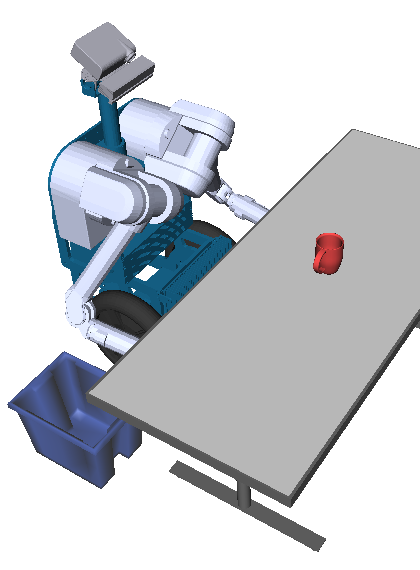
\includegraphics[width=1.7cm]{figs/herbbin/step0cropped.png}
%         \;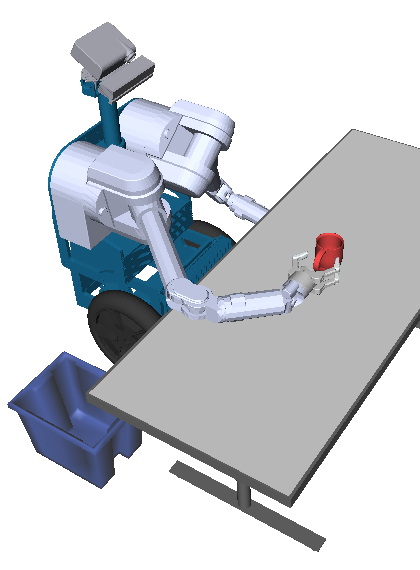
\includegraphics[width=1.7cm]{figs/herbbin/step01cropped.png}};
%
%      \node at ( 6,2.5) {\includegraphics[width=9cm]{build/multistep-prescribed/herbbinnom-g1ll}};
%      
%   \end{tikzpicture}
%\end{frame}

\begin{frame}
   \frametitle{Maximizing Utility: Workcell Experiments}
   \begin{tikzpicture}[font=\small]
      \tikzset{>=latex} % arrow heads
      \draw[step=1,black!15,very thin,opacity=\gridopacity] (0,0) grid (12,8);

      %\node at ( 6,6.5) {
      %   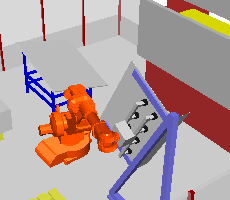
\includegraphics[width=2.7cm]{figs/workcell/cropped-config-f.png}
      %   \;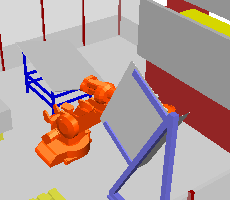
\includegraphics[width=2.7cm]{figs/workcell/cropped-config-g.png}};

      \node[inner sep=0pt] (vidnode) at (6,6.5) {%
         \href{\tikzvidtarget{incbi-roadne}}{%
         \includegraphics[width=4cm]{videos/workcell-cropped.png}}};
      \tikzvidplayat{incbi-roadne}{vidnode}{videos/workcell-cropped.mp4}{}

      \node at ( 6,2.5) {\includegraphics[height=4cm]{build/multistep-prescribed/workcell-g1ll-lemuronly}};
      
   \end{tikzpicture}
\end{frame}
